
\begin{frame}{Recorrido UPV Virtual en teléfonos inteligentes}
%\begin{block}{Recorrido UPV Virtual en teléfonos inteligentes} 
Demo incremental, que emplea OpenGL ES 2.0 (compatible con el 100\% de los smartphones). 
\begin{itemize}
\item Versión 1: Solo mundo virtual (no inmersivo). El usuario se movía con presionando teclas de la interfaz de usuario
\item Versión 2: Mundo virtual inmersivo (integrado a unos lentes). El usuario movía la vista mediante los datos obtenidos por el sensor giroscopio del teléfono inteligente y avanzaba usando un manos libres alámbrico.
\item Versión 3: Controlado por voz. El usuario se movía dentro del entorno mediante comandos de voz.
\item Versión 3.5: Controlado mediante control de videojuegos (Bluetooth o USB)
\end{itemize}
%\end{block} 
\end{frame}

\renewcommand{\EntradaBibtex}{Reporte2019}
\begin{frame}{\citetitle{\EntradaBibtex} \footnotemark[1] (1)}

%\begin{frame}{Recorrido UPV Virtual 1.0\footnotemark }
%\begin{block}{} 
\begin{columns}
\begin{column}{0.48\textwidth}
    \begin{center}

\begin{itemize}
\item La navegación es mediante botones (adelante, atrás, izquierda, derecha, subir, bajar)
\item Una potencial mejora es mediante eventos de toque en pantalla
\end{itemize}
     \end{center}

\end{column}
\begin{column}{0.52\textwidth}  
    \begin{center}
\begin{itemize}
\end{itemize}
     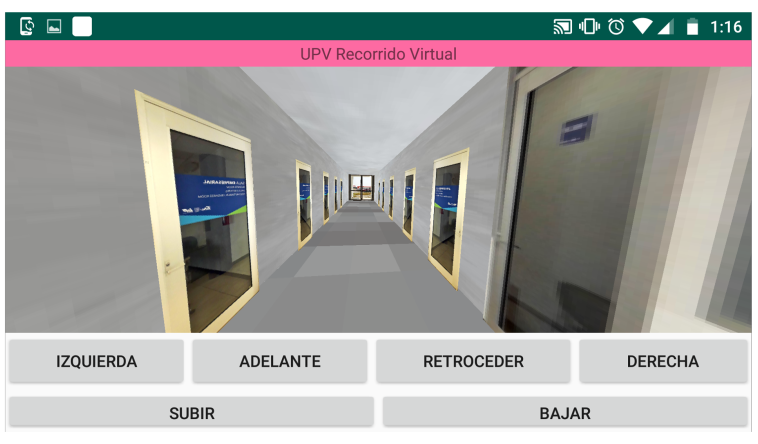
\includegraphics[width=0.9\textwidth]{Figs/RecorridoUPV_V1}\\
     \end{center}
\end{column}
\end{columns}
%\end{block} 
\footnotetext[1]{\fullcite{\EntradaBibtex}}
%\footnotetext{Baez Zapata Marıa Fernanda, Cárdenas Castillo Jesús Alfredo, Olvera Osuna José Armando and Wang Yu Hsiang. \textbf{Recorrido UPV en Android}. Proyecto Final de la Asignatura ``Cómputo en Dispositivos Móviles'', 2019. Sin Publicar.}
%\\setcounter{footnote}{0}
\end{frame}


%\begin{frame}{Recorrido UPV Virtual 1.0 (2)}
%\renewcommand{\EntradaBibtex}{Reporte2019}
\begin{frame}{\citetitle{\EntradaBibtex}  (2)}
%\begin{block}{Recorrido UPV Virtual 1.0 (2)} 
\begin{itemize}
\item Vistas de los diferentes edificios
\end{itemize}
    \begin{center}
     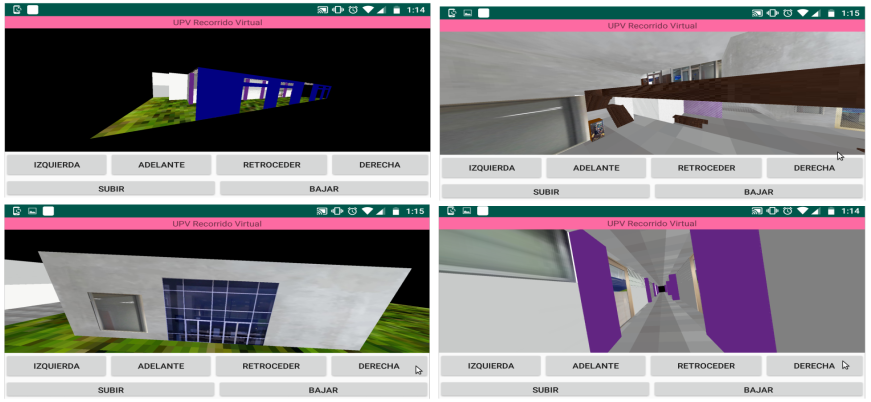
\includegraphics[width=0.80\textwidth]{Figs/RecorridoUPV_V2}\\
     \end{center}
%\end{block} 
\end{frame}

\renewcommand{\EntradaBibtex}{RecorridoVirtualLentesVR_2019}
%\begin{frame}{Recorrido UPV Virtual 2.0\footnotemark}
\begin{frame}{\citetitle{\EntradaBibtex}  (2)}
%\begin{block}{Recorrido UPV Virtual 2.0\footnotemark} 
\begin{columns}
\begin{column}{0.48\textwidth}
    \begin{center}

\begin{itemize}
\item Se extendió el demo 1.0 para generar una vista dual, requerida para su uso en conjunto con un armazón de VR.
\item La vista cambia en base a lo obtenido por el giroscopio, y el movimiento se controla mediante el botón del manos libres.
\end{itemize}
     \end{center}

\end{column}
\begin{column}{0.52\textwidth}  
    \begin{center}
\begin{itemize}
\end{itemize}
     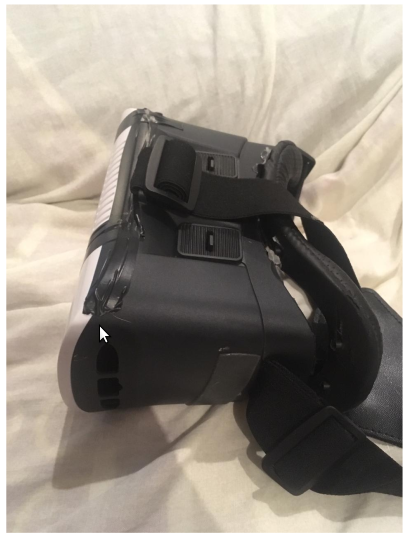
\includegraphics[width=0.4\textwidth]{Figs/RecorridoUPV_V3}\\
     \end{center}
\end{column}
\end{columns}
%\end{block} 
%\footnotetext{\fullcite{RecorridoVirtualLentesVR_2019}}
\footnotetext[1]{\fullcite{\EntradaBibtex}}
%\footnotetext{Alarcon Longoria Carlos Alberto, Alonso Cepeda Leonardo Daniel and Torres Grimaldo Luis Angel. \textbf{Recorrido UPV Virtual en Android}.  Proyecto Final de la Asignatura ``Cómputo en Dispositivos Móviles'', 2019. Sin Publicar.}
%\\setcounter{footnote}{0}
\end{frame}


\renewcommand{\EntradaBibtex}{RecorridoVirtualLentes_ComandosVoz2020}
\begin{frame}{\citetitle{\EntradaBibtex}  (1)}
%\begin{block}{Recorrido UPV Virtual 3.0\footnotemark} 
\begin{columns}
\begin{column}{0.48\textwidth}
    \begin{center}
\begin{itemize}
\item Se eliminó el uso del botón del manos libres para incluir comandos de voz
\item La aplicación respondía a los comandos de voz, de tal forma que el usuario no debería mover nada
\end{itemize}
     \end{center}

\end{column}
\begin{column}{0.52\textwidth}  
    \begin{center}
     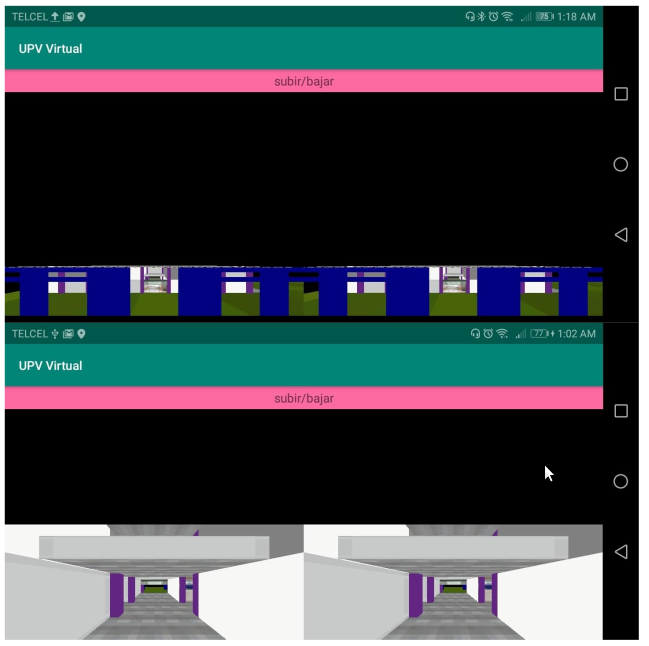
\includegraphics[width=0.6\textwidth]{Figs/RecorridoUPV_V5}\\
     \end{center}
\end{column}
\end{columns}
%\end{block} 
\footnotetext[1]{\fullcite{\EntradaBibtex}}
%\footnotetext{José Treviño Olvera. \textbf{Recorrido UPV Virtual en Android con Controles de Voz.}  Proyecto Final de la Asignatura. ``Cómputo en Dispositivos Móviles'', 2020. Sin Publicar.}
%\\setcounter{footnote}{0}
\end{frame}

\renewcommand{\EntradaBibtex}{RecoridoUPV_controles_2021}
%\begin{frame}{Recorrido UPV Virtual 3.5 \footnotemark}
%\begin{block}{Recorrido UPV Virtual 3.5 \footnotemark } 
\begin{frame}{\citetitle{\EntradaBibtex}  (1)}
\begin{itemize}
\item Se incorporaron varios controles de consolas de videojuego para la navegación.
\end{itemize}
\begin{columns}
\begin{column}{0.48\textwidth}
\begin{center}
	\begin{tabular}{ccc}
		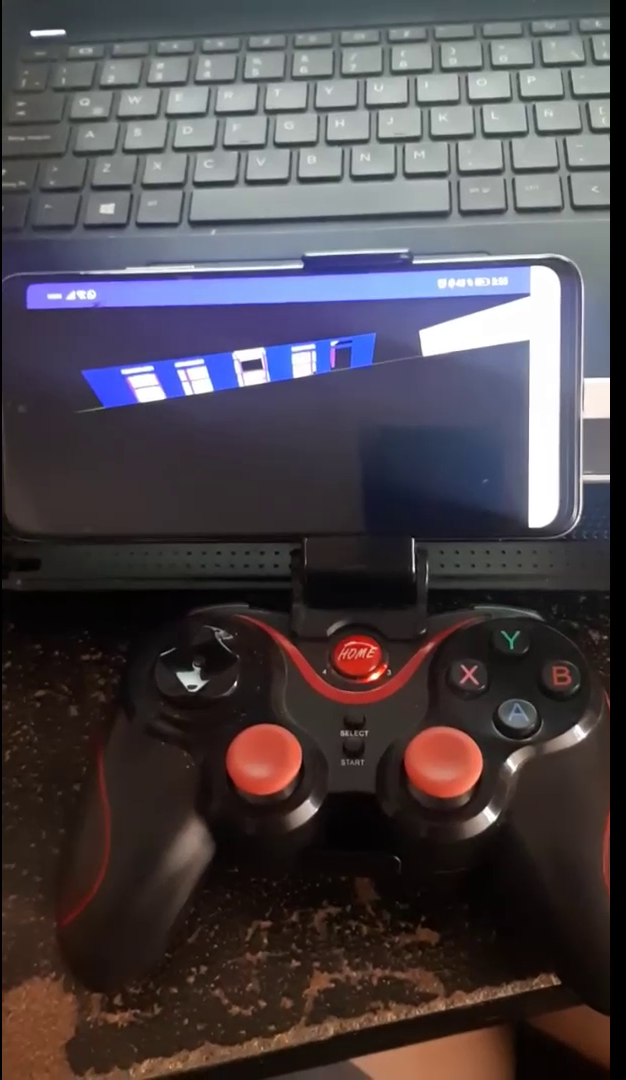
\includegraphics[width=0.25\linewidth]{Figs/UPV_Control01} & 		
		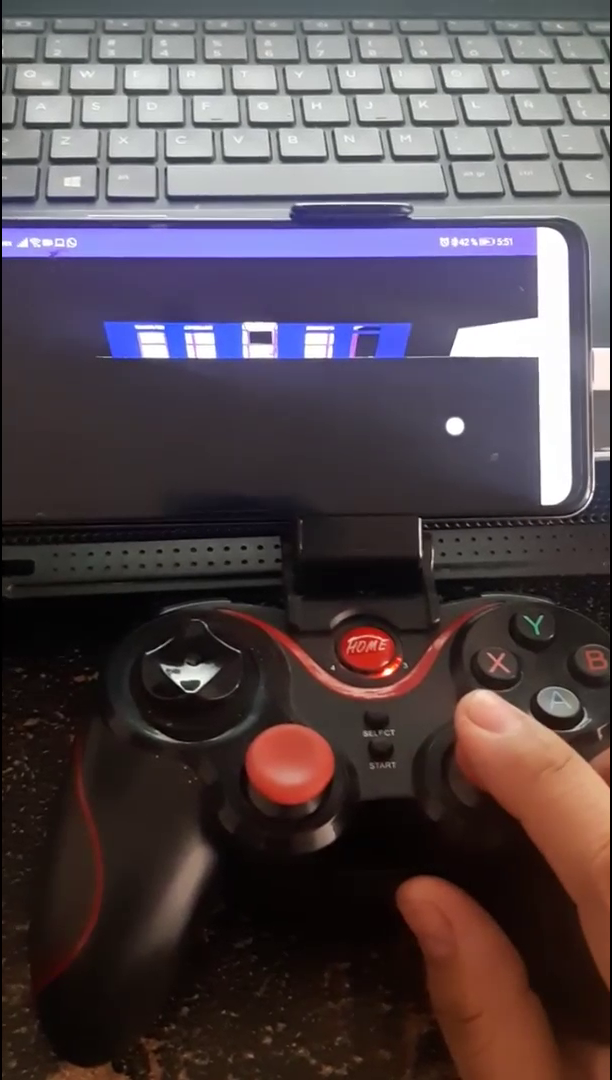
\includegraphics[width=0.25\linewidth]{Figs/UPV_Control02} & 
        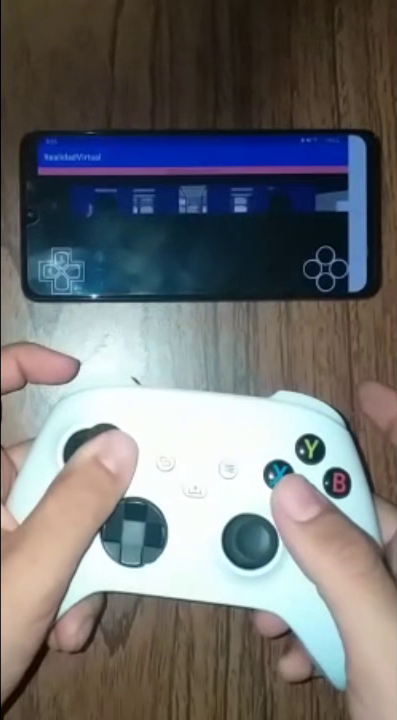
\includegraphics[width=0.25\linewidth]{Figs/UPV_Control04}\\
	\end{tabular}
\end{center}
\end{column}
\begin{column}{0.48\textwidth}
\begin{center}
	\begin{tabular}{c}
		    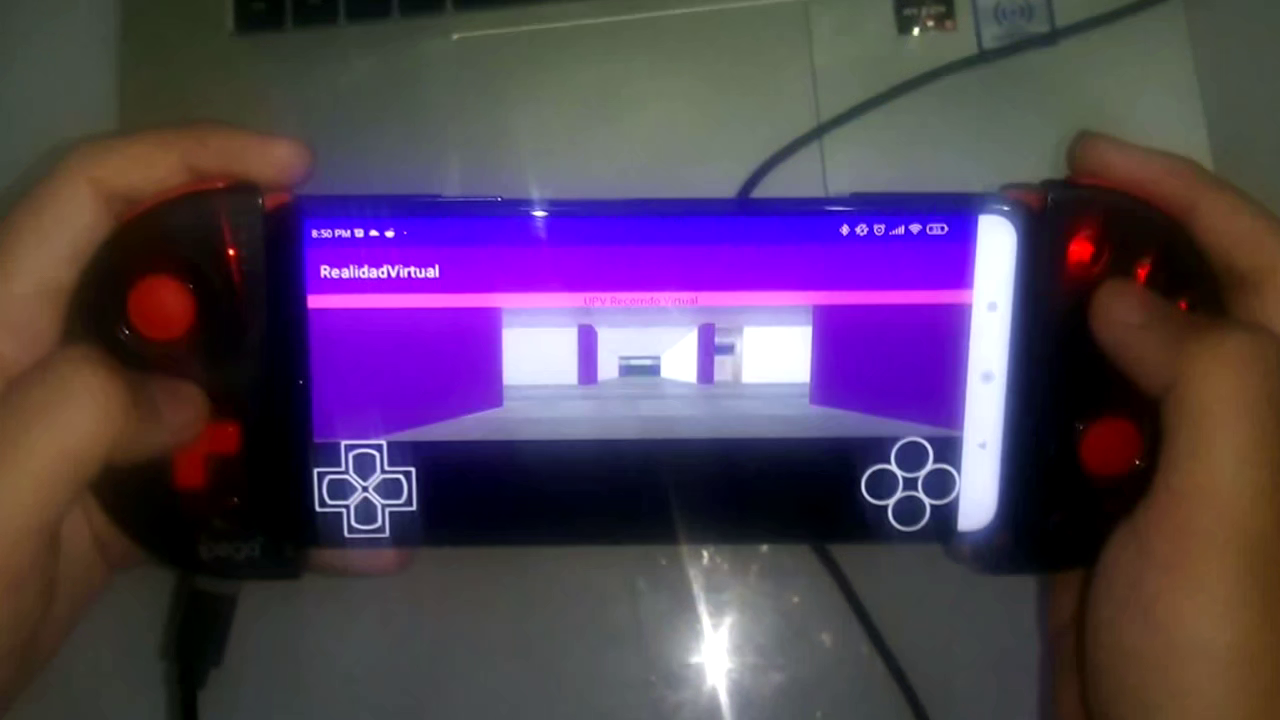
\includegraphics[width=0.45\linewidth]{Figs/UPV_Control03}\\
		    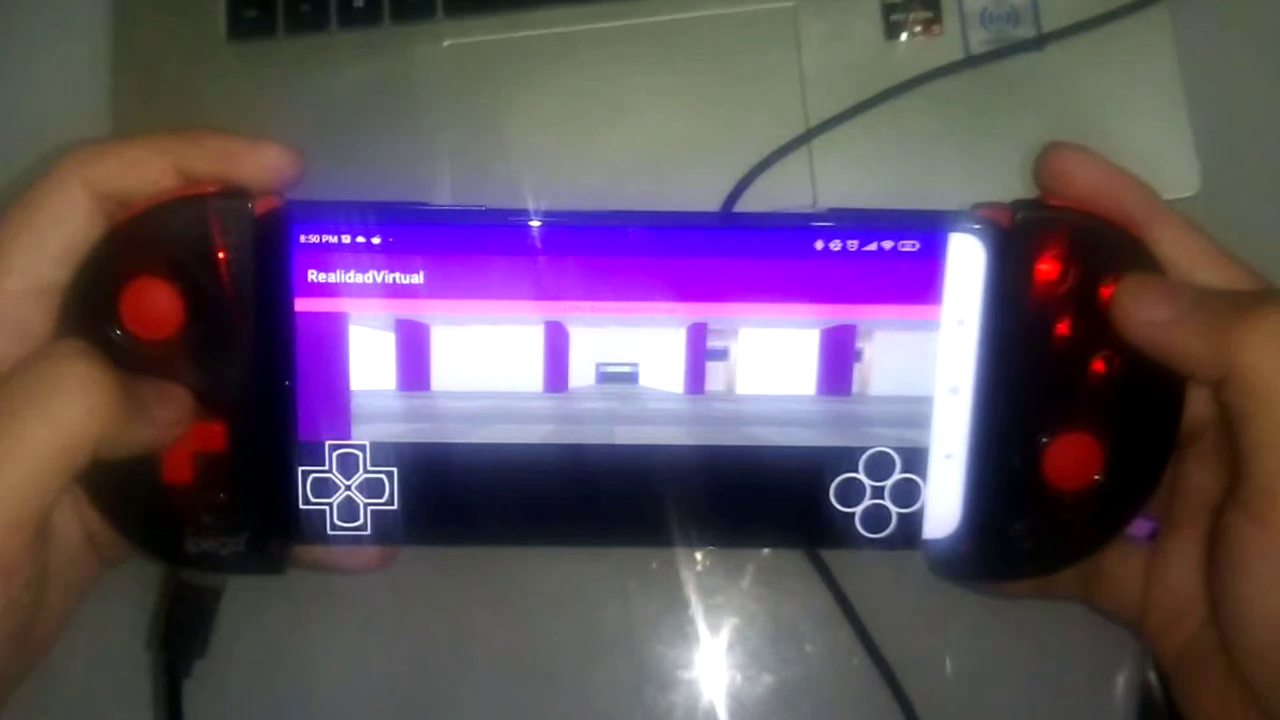
\includegraphics[width=0.45\linewidth]{Figs/UPV_Control05}\\
	\end{tabular}
\end{center}	
\end{column}
\end{columns}
%\end{block} 
\footnotetext[1]{\fullcite{\EntradaBibtex}}
%\footnotetext{\fullcite{RecoridoUPV_controles_2021}}
\end{frame}

